\documentclass[a4paper]{scrreprt}

% Uncomment to optimize for double-sided printing.
% \KOMAoptions{twoside}

% Set binding correction manually, if known.
% \KOMAoptions{BCOR=2cm}

% Localization options
\usepackage[english]{babel}
\usepackage[T1]{fontenc}
\usepackage[utf8]{inputenc}

% Quotations
\usepackage{dirtytalk}

% Floats
\usepackage{float}

% Enhanced verbatim sections. We're mainly interested in
% \verbatiminput though.
\usepackage{verbatim}

% Automatically remove leading whitespace in lstlisting
\usepackage{lstautogobble}

% CSV to tables
\usepackage{csvsimple}

% PDF-compatible landscape mode.
% Makes PDF viewers show the page rotated by 90°.
\usepackage{pdflscape}

% Advanced tables
\usepackage{array}
\usepackage{tabularx}
\usepackage{longtable}

% Fancy tablerules
\usepackage{booktabs}

% Graphics
\usepackage{graphicx}

% Current time
\usepackage[useregional=numeric]{datetime2}

% Float barriers.
% Automatically add a FloatBarrier to each \section
\usepackage[section]{placeins}

% Custom header and footer
\usepackage{fancyhdr}

\usepackage{geometry}
\usepackage{layout}

% Math tools
\usepackage{mathtools}
% Math symbols
\usepackage{amsmath,amsfonts,amssymb}
\usepackage{amsthm}
% General symbols
\usepackage{stmaryrd}

% Utilities for quotations
\usepackage{csquotes}

% Bibliography
\usepackage[
  style=alphabetic,
  backend=biber, % Default backend, just listed for completness
  sorting=ynt % Sort by year, name, title
]{biblatex}
\addbibresource{references.bib}

\DeclarePairedDelimiter\abs{\lvert}{\rvert}
\DeclarePairedDelimiter\floor{\lfloor}{\rfloor}

% Bullet point
\newcommand{\tabitem}{~~\llap{\textbullet}~~}

\pagestyle{plain}
% \fancyhf{}
% \lhead{}
% \lfoot{}
% \rfoot{}
% 
% Source code & highlighting
\usepackage{listings}

% SI units
\usepackage[binary-units=true]{siunitx}
\DeclareSIUnit\cycles{cycles}

\newcommand{\lecture}{41109 - Privacy and Data Security}
\newcommand{\series}{07}
% Convenience commands
\newcommand{\mailsubject}{\lecture - Series \series}
\newcommand{\maillink}[1]{\href{mailto:#1?subject=\mailsubject}
                               {#1}}

% Should use this command wherever the print date is mentioned.
\newcommand{\printdate}{\today}

\subject{\lecture}
\title{Series \series}

\author{Michael Senn \maillink{michael.senn@students.unibe.ch} --- 16-126-880}

\date{\printdate}

% Needs to be the last command in the preamble, for one reason or
% another. 
\usepackage{hyperref}

\begin{document}
\maketitle


\setcounter{chapter}{\numexpr \series - 1 \relax}

\chapter{Series \series}

\section{Differential privacy --– Theory}

Recall the definition of $\epsilon$-differential privacy for a probabilistic
algorithm $M: X^n \rightarrow Y$, if for every $Y' \subset Y$ and neighbouring
datasets $X, X'$:

\[
  P[M(X^n) \in Y'] \leq \exp(\epsilon) \cdot P[M(X'^n) \in Y']
\]

We will try to approximate this as follows. Let $x \in Y = \{0, 1\}$, then:
\begin{align*}
  P[M(X^n) = x] & = \delta \cdot P[x_i = x] + (1 - \delta) \cdot P[R = x] \\
                & = \delta \cdot P[x_i = x] + (1 - \delta) \cdot \frac{1}{2} \\
                & = \delta \cdot P[x_i = x] + \frac{1 - \delta}{2}
\end{align*}

Similarly:
\begin{align*}
  P[M(X'^n) = x] & = \delta \cdot P[x'_1 = x] + (1 - \delta) \cdot P[R = x] \\
                 & = \delta \cdot \left(\frac{n-1}{n} \cdot P[x_1 = x] + \frac{1}{n} \cdot (1 - P[x_1 = x]\right) + (1 - \delta) \cdot \frac{1}{2} \\
                 & = \delta \cdot \left(\frac{n-1}{n} \cdot P[x_1 = x] + \frac{1}{n} \cdot (1 - P[x_1 = x]\right) + \frac{1 - \delta}{2}
\end{align*}

In order to find an upper bound for the fraction, we will try to find an upper
bound for the nominator, and a lower bound for the denominator:
\begin{align*}
  P[M(X^n) = x] & \leq \delta + \frac{1 - \delta}{2} & \text{For } P[x_1 = x] = 1 \\
  P[M(X'^n) = x] & \geq \frac{\delta}{n} + \frac{1 - \delta}{2} & \text{For } P[x_1 = x] = 0
\end{align*}

And thus:
\begin{align*}
  \frac{P[M(X^n) = x]}{P[M(X'^n) = x]} & \leq \frac{\frac{1-\delta}{2}}{\frac{\delta}{n} + \frac{1-\delta}{2}} \\
                                       & = \frac{1 - \delta}{\frac{2 \delta}{n} + 1 - \delta} \\
                                       & = \frac{-2 \delta}{2 \delta + n  - \delta \cdot n} + 1 \\
                                       & \approx 1 & \text{For large } n
\end{align*}

As $n - \delta \cdot n$ diverges, for $\delta \in [0, 1)$. Then:

\begin{align*}
  \frac{P[M(X^n) = x]}{P[M(X'^n) = x]} & \approx \exp\left(\frac{-2 \delta}{2 \delta + n - \delta \cdot n}\right)
\end{align*}

And hence:
\begin{align*}
  \epsilon \approx \frac{-2 \delta}{2 \delta + n - \delta \cdot n} \approx \frac{1}{n}
\end{align*}

\section{Differential privacy --– Privacy}

Based on the supplied data, differentially-private histograms for $\epsilon \in
\{0.1, 0.5, 2\}$ were calculated using the Laplace mechanism. It is evident
that, for small epsilon values, the resulting histogram has little in common
with the actual distribution wheras for large values the sanitized distribution
is very similar to the actual distribution.

As such a large value of epsilon --- while offering lower differential privacy
--- is likely much more useful for statistical purposes.

The figures below show some of the results for three different epsilon values
as well as the original distribution. The code used to generate them is
available as an attached Jupyter notebook.

\begin{figure}
  \centering
  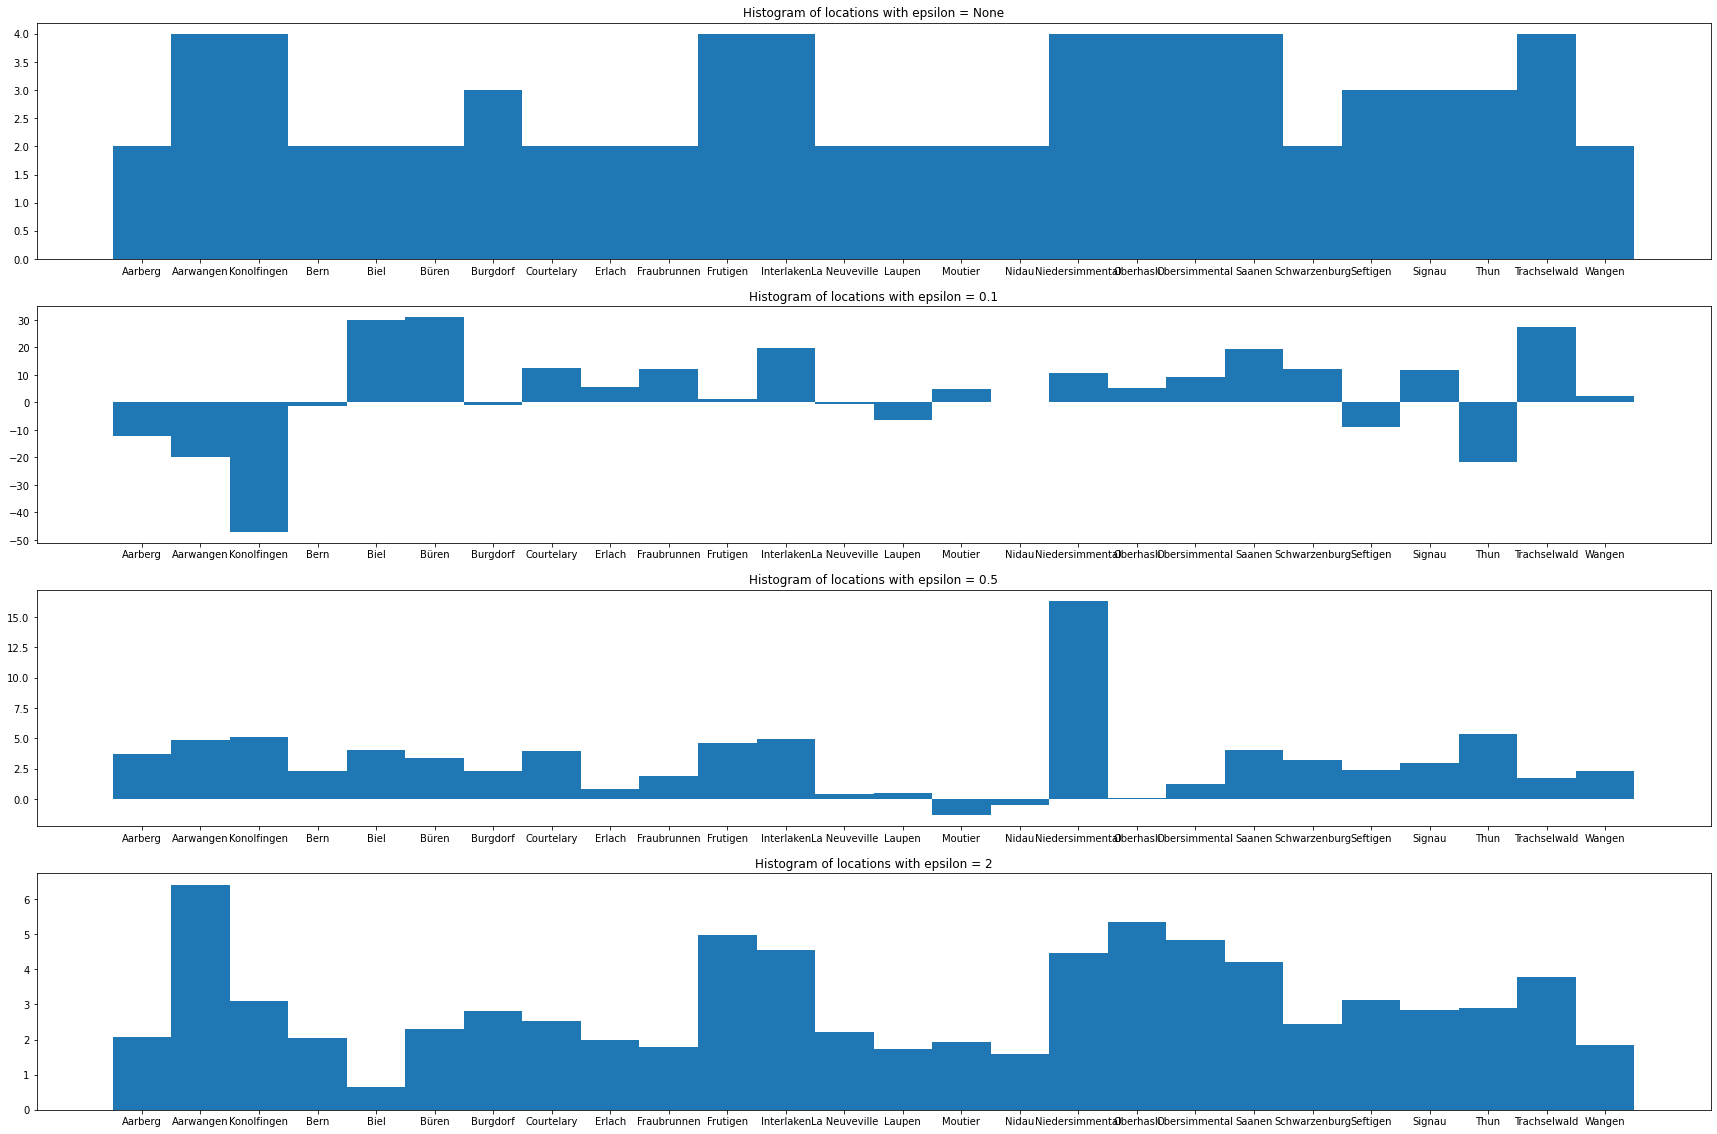
\includegraphics[width=\textwidth]{resources/2_location.png}
  \caption{DP sanitization of location distribution}
\end{figure}

\begin{figure}
  \centering
  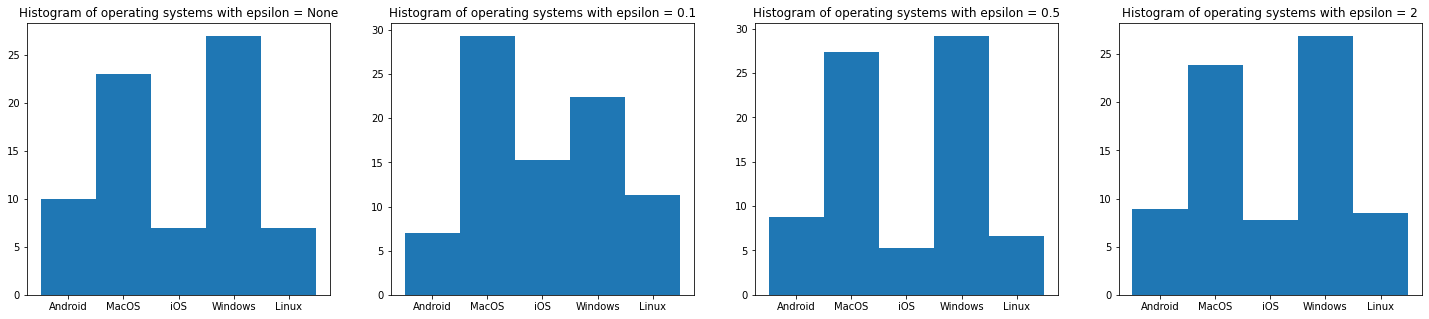
\includegraphics[width=\textwidth]{resources/2_system.png}
  \caption{DP sanitization of operating system distribution}
\end{figure}

\begin{figure}
  \centering
  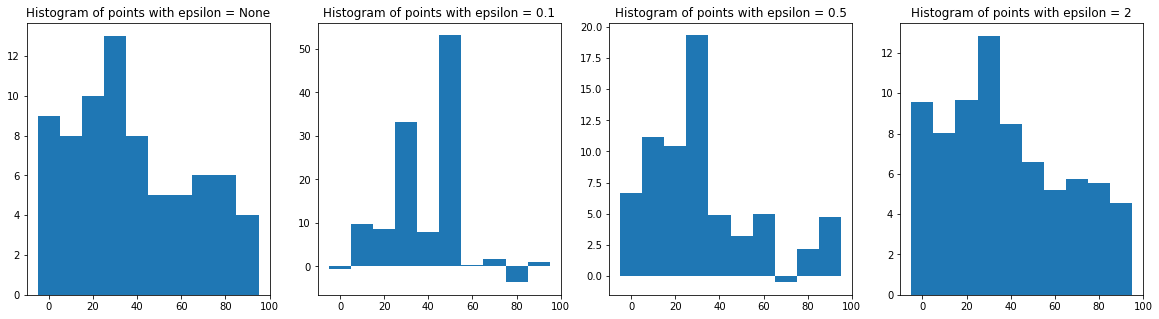
\includegraphics[width=\textwidth]{resources/2_points.png}
  \caption{DP sanitization of points distribution, using a bin width of 10}
\end{figure}

\printbibliography

\end{document}
